\section{Example}
\label{sec:comparison_with_EMV2}

To illustrate some of the key differences between our approach and approaches that explicitly enumerate and propagate faults such as the AADL Error Model Annex, Version 2 (EMV2)~\cite{EMV2}, we use a simplified example based on the Wheel Brake System (WBS) adapted from ~\cite{WBS_EMV2_Example}.

As shown in Figure~\ref{fig:comparison_with_EMV2}, a simplified WBS system takes the output signal from the Pedal component, passes through the Sensor and the Braking System Control Unit (BSC) components, and generates a pressure output from the Valve component to apply to the Wheels. To assist explanation in a modeling setting, we use the general term "fault" to denote all component errors, hardware failures, and system faults captured by both approaches.

In an EMV2 approach, all faults have to be explicitly propagated through each component (e.g., applying fault types on the out ports) in order for a component to have an impact on the rest of the system. The fault types are descriptive in that they cannot be processed directly by any behavioral analysis; the meaning of the fault types have to be explicitly interpreted in the form of data to be analyzed. Consequently, there is no behavioral analysis on the EMV2 model. At the system level, the tool can aggregate the fault flow and propagation information from different components to compose an overall fault flow diagram or fault tree.

In the Safety Annex approach, faults are not discrete entities artificially tagged and propagated (as the other approach), but captured as faulty behaviors (in Safety Annex) that augment the system's behavioral model (in AGREE). No separate or explicit propagation through the components is done for the faults; all behavioral propagations (e.g., how inputs are passed to the outputs) are modeled in AGREE no matter the inputs are normal or faulty. Users can apply formal behavioral analysis on the model and verify if system level properties hold with or without the presence of faults.

\begin{figure}[h!]
	\vspace{-0.19in}
	\centering
	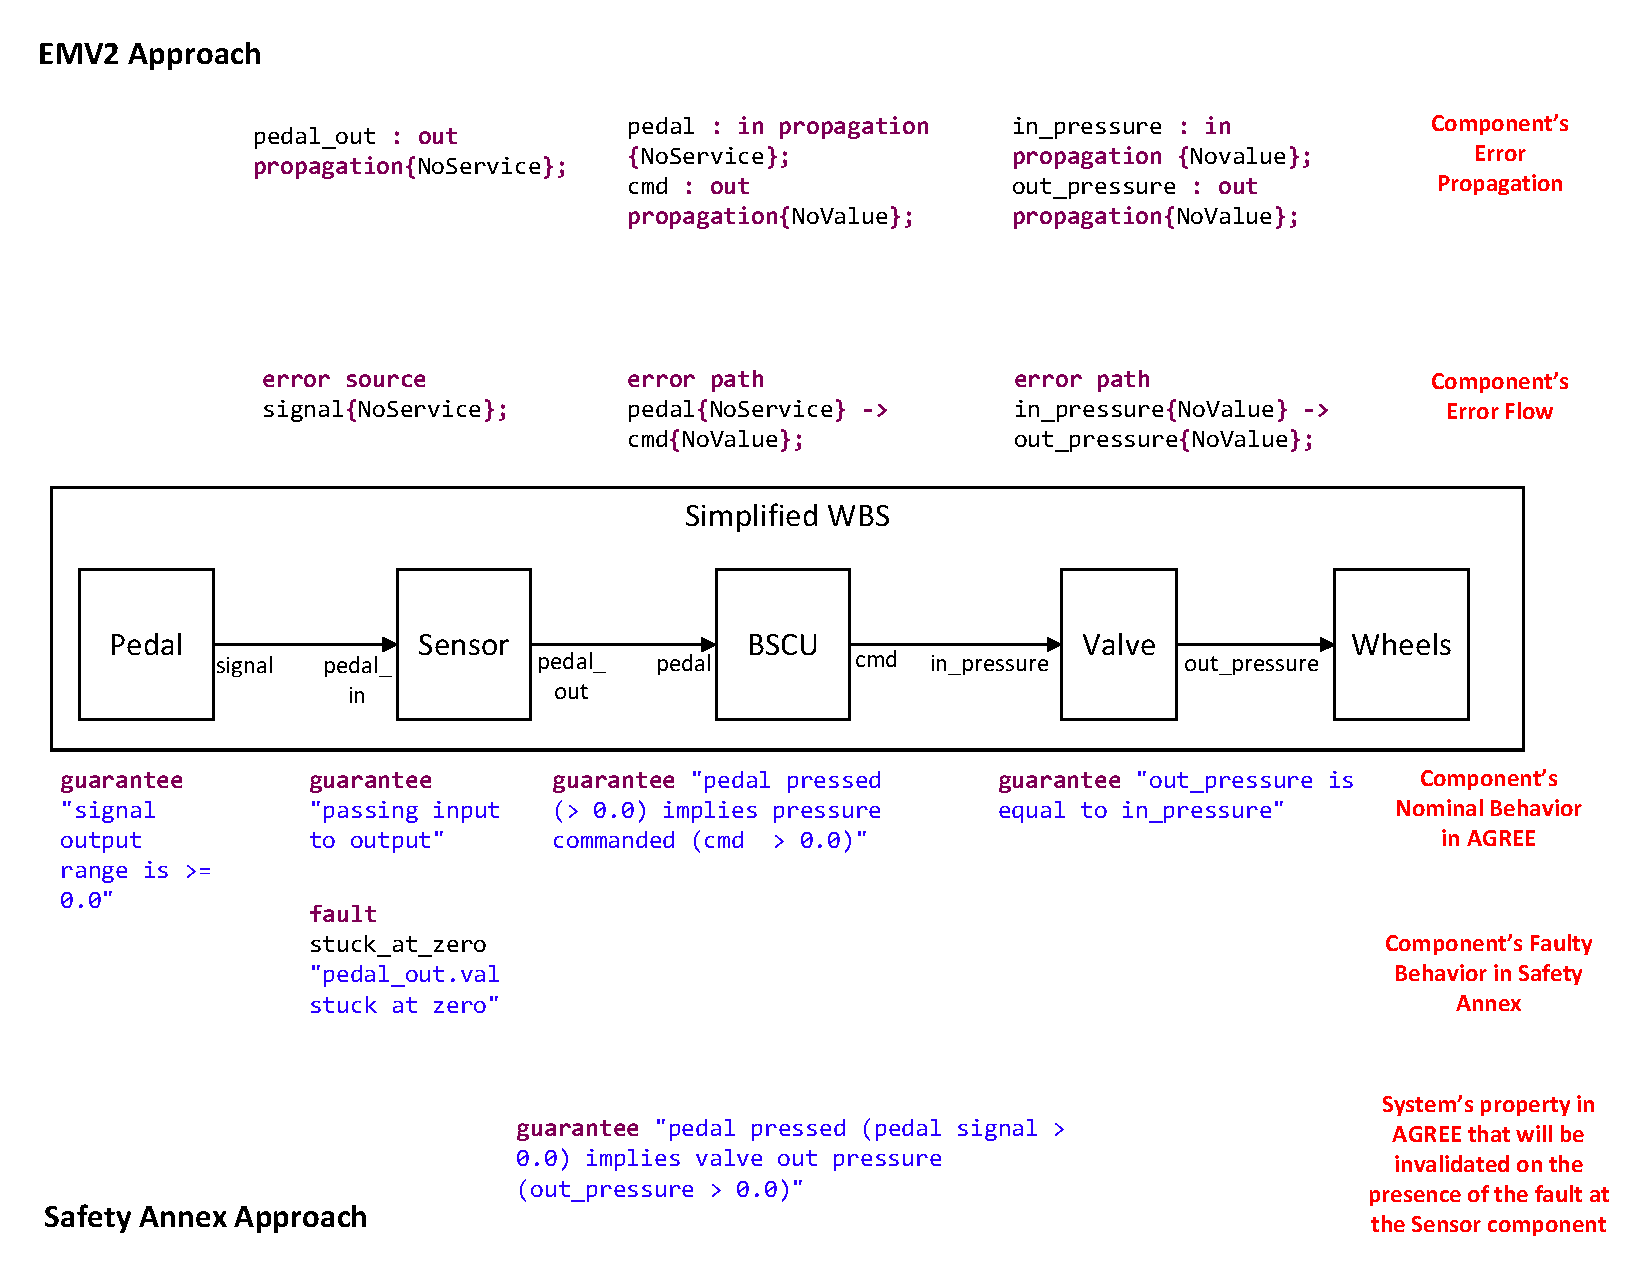
\includegraphics[trim=0 9 0 5,clip,width=0.85\textwidth]{images/Visio-Comparison_with_EMV2.pdf}
	%\vspace{0.4in}
	\caption{Differences between Safety Annex and EMV2}
	\label{fig:comparison_with_EMV2}
\end{figure}

 


